\documentclass[10pt]{article}
\usepackage[T1]{fontenc}
\usepackage[margin=0.85in]{geometry}
\usepackage{amsmath,amssymb,booktabs,graphicx,hyperref,xurl}
\hypersetup{hidelinks}
\setlength{\emergencystretch}{2em}
\clubpenalty=10000
\widowpenalty=10000
\title{Executable Recovery Service under Physical KV and Peer Constraints}
\author{A-line research working draft}
\date{2 October 2026}
\begin{document}
\maketitle
\begin{center}\textbf{Exploratory native results; adaptive quantum benefit is not established.}\end{center}
\begin{abstract}
Recovering a paused language-model request requires capacity for restoration, subsequent KV growth, and actual execution. A native 128-request comparison shows that ordinary free-fit backfill leaves a substantial output-pause tail: funded recovery reduces the 95th percentile of per-request maximum gaps from 3.885 to 1.575 seconds, at 1.52\% lower actual output rate and 1.85\% higher mean completion flow. Individual requests can nevertheless lose several seconds. Motivated by observed re-eviction after short service, we implement a recovery lease coupling a protected output quantum to physical endpoint capacity, execution reservations, and selective peer admission. Two complete lease comparisons do not establish stable superiority for recovery-cost-ratio adaptation. Adaptive is worse than fixed4 in the first run group (P95 gaps 1.708 versus 1.492 seconds); reversing run order reverses the gap and throughput rankings (P95 1.401 versus 1.570 seconds), while adaptive mean flow is worse in both groups. Natural-ending development controls match within each capacity block, but independent holdout arms differ: native scores 10/16 exact match versus 8--9/16 for the other arms. No recovery-policy action activates in any task block, so these quality differences cannot establish a quantum effect. The evidence supports an executable resource condition and a conditional progress argument, but not a reliably beneficial adaptive rule. We stop developing this particular cost-ratio formulation and retain peer displacement and remaining-work information as the next research question.
\end{abstract}

\section{Question, objective, and evidence scope}
With finite GPU KV and compute capacity, how should recovery, eviction, and continuous service be coordinated to shorten long output stalls while controlling throughput, completion time, and peer costs?

The primary metric is $\operatorname{P95}(g_i)$, where $g_i$ is the largest interval between distinct host output receipts after first output. We also retain the full gap distribution, maximum gap, actual returned tokens per capture second, arrival-to-completion flow, TTFT, and complete-request goodput on a fixed development TTFT/gap frontier. TTFT is not included in $g_i$; moving a wait before first output can improve this metric without improving completion. Client receipt and device production times are not separately measured.

Current evidence has three parts: a complete-cohort tail/cost tradeoff against an active ordinary backfill baseline; a native implementation of a physical-capacity and execution condition for recovery service; and a two-run comparison in which the adaptive/fixed4 service ordering changes. The strong-baseline block has one run per arm; the lease comparison has two run groups, with reversed serial order, on the same already-seen input. Events and requests within it are not independent run-level repeats. These results do not establish statistical stability, independent novelty, or paper readiness.

\section{Observation motivating the resource condition}
An earlier R02 native run reduced P95 gaps from 7.939 to 1.552 seconds with funded Q1, while actual output rate fell 0.67\% and actual preemptions rose from 46 to 103. This historical block ran on a different physical GPU from the new comparisons and is used only as motivation.

A focused raw-output join finds 48 re-evictions among its 58 recovery episodes on 21 source requests: 32 fund another recovery and 16 are native preemptions. Median service before re-eviction is 19 new outputs; 12 episodes receive at most nine. All six short native re-evictions retain unused slots in owned KV pages. Two one-output cases retain 12 and nine slots, yet their subsequent gaps differ sharply: 1.233 and 0.152 seconds. Unused slots expose an execution opportunity, not a counterfactual benefit.

Three candidate actions follow: commit restoration through first output as one operation; choose the recovery service quantum with its growth and peer costs; or schedule around currently known releases. Existing Q1 already implements much of the first, and a previous hard-cap release-deferral pilot failed its service objective. We implement the second, while testing fixed quanta on the identical resource path to distinguish quantum selection from admission repair.

\section{Model and executable decision}
For target $i$, observe prompt length $P_i$, attained outputs $O_i$, known cap $M_i$, physically owned blocks $H_i$, free blocks $F$, native in-flight reservations $R$, and current output ages $a_i,a_j$ of other live output-bearing requests. Transfer state and native eligibility remain necessary. Block size is $B$. Neither future EOS nor realized future output length is available to the policy.

For $q$ further outputs, endpoint capacity and unowned growth are
\begin{equation}
K_i(q)=\left\lceil\frac{P_i+O_i+q-1}{B}\right\rceil,
\qquad G_i(q)=\max(0,K_i(q)-H_i).
\end{equation}
The final generated token has not yet been computed into KV, explaining the $-1$. After a proposed victim releases verified private blocks, require $G_i(q)\le F-R$, using current physical ownership and the installed scheduler's allocation semantics. A peer requiring $C_j$ additional blocks is admitted only when $G_i(q)+R+C_j\le F$, with already-accounted reservations counted once. Recheck after native scheduling as ownership changes. A promise covering restoration alone can become invalid at the next page boundary.

Let $h$ and $d$ be rolling-median estimates of past host recovery overhead and decode interval. The completed-episode sample runs from protection start, before native admission, to first-output observation; subtracting one prior decode interval estimates $h$. This includes queueing, transfer and execution and is not a DMA measurement. Unknown estimates select Q1. With the exploratory peer-age reference $L=\max(1\mathrm{s},a_i)$, optional service uses
\begin{equation}
T(q)=h+qd,\qquad \max_j a_j+T(q)\le L.
\end{equation}
The adaptive rule seeks the smallest integer $q$ with $h/(h+qd)\le\rho$, then truncates it by physical capacity, peer headroom, remaining output cap and a quantum ceiling. Here $\rho=0.5$ and $q\le16$. If optional service is infeasible, established Q1 progress takes precedence. Consequently an overdue peer may still wait: the estimated age condition is not a hard SLO.

Choose $q$ and endpoint capacity before funding and recheck at commit. During loading and execution, reserve remaining growth, one compute token and, until the target runs, one running slot. Preserve the native load path and admit compatible peers selectively. Logical resource deferrals return to the ordinary waiting queue independently of real asynchronous loads. Completion, the output goal, a newly urgent peer, or a changed necessary condition releases optional protection.

This admission distinction matters: an older Q10 interval blocked every non-target waiter, including 174 numerically fitting heads, and failed service comparisons despite fewer preemptions. All new Q1, fixed4 and adaptive arms therefore share the repaired resource and admission path; a comparison only with the older Q1 path would confound these changes.

\paragraph{Conditional progress.}
Suppose restoration has completed, a nonterminal target remains natively eligible and receives one valid decode token on every successful decoder call, full $q$-output growth remains reserved without double spending, physical ownership and transfer state stay valid, and the lease remains active without revocation. Then it produces $q$ outputs within $q$ successful decoder calls, or terminates earlier. Indeed, $K_i(k)\le K_i(q)$ supplies capacity for every $k\le q$, and each valid call advances output. This local property does not bound restoration, kernel duration, scheduling delay, failure, or revocation. The implemented policy may voluntarily release after Q1 when peer age or growth conditions change; it therefore does not promise an unconditional $q$ outputs beyond Q1. The statement is not a wall-clock guarantee, and the estimated peer condition is not a theorem about future age.

\section{Completed native comparisons}
The new blocks use the same RTX 5090 endpoint, OLMoE-1B-7B-0924 in BF16, native KV saving, 4,096 usable GPU blocks of 16 tokens, 16 GiB host KV, and a maximum of 32 running requests. Each article arm completes all 128 requests. The strong-baseline and lease blocks have separate run groups and implementations. We use within-block comparisons, retain both lease run groups, and do not pool their events as replicates (Figure~\ref{fig:results}).

\begin{figure}[t]
\centering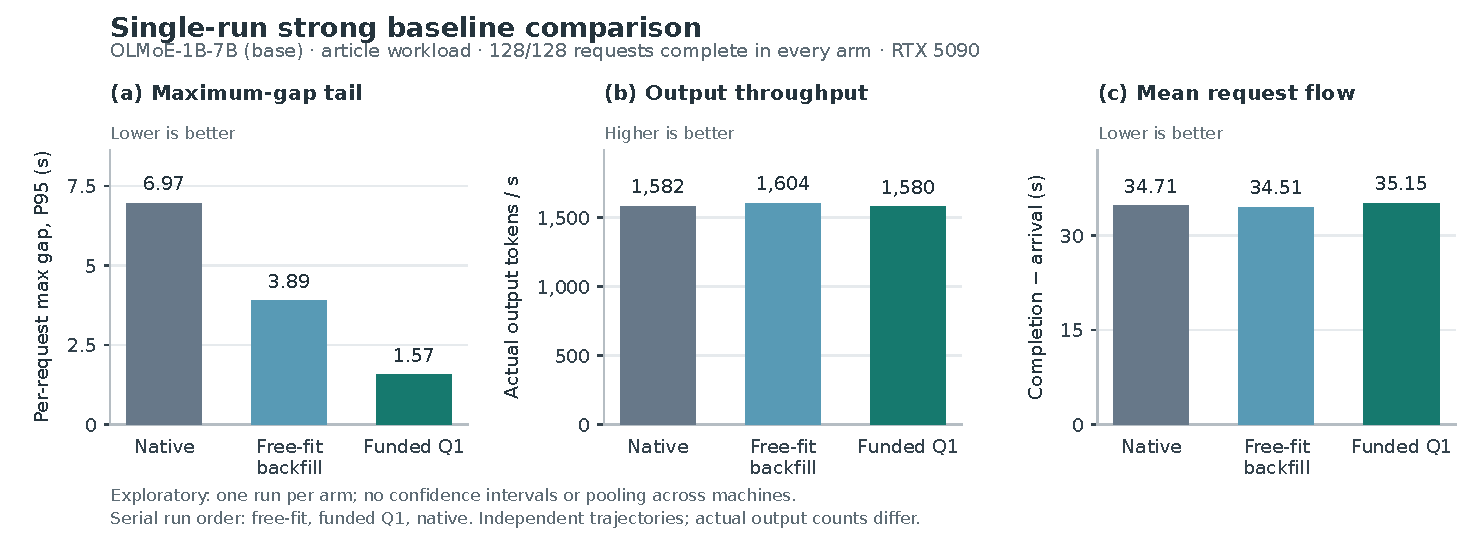
\includegraphics[width=\linewidth]{../output/newhost_results.pdf}
\caption{The completed strong-baseline group tests native scheduling, ordinary free-fit and the existing funded Q1 path. Each bar is one complete 128-request run. Lease comparisons use a separate resource/admission implementation and are shown in Figure~\ref{fig:repeat}; cross-group differences do not isolate a quantum effect.}
\label{fig:results}
\end{figure}

\paragraph{Ordinary free-fit leaves a tail residual.}
Native, ordinary and funded Q1 have P95 gaps of 6.965, 3.885 and 1.575 seconds; maxima are 11.068, 10.874 and 2.044 seconds. Ordinary makes 20 actual native asynchronous-load admissions, all followed by output and completion, without a same-call preemption. Thus the comparator is active. All predeclared completion, mechanism and service checks pass, including at least 97\% relative output rate and at most 105\% mean flow for the specified pairs.

Relative to ordinary, funded Q1 loses 1.52\% actual output rate and adds 1.85\% mean flow; relative to native these costs are 0.13\% and 1.28\%. Preemptions are 43, 59 and 102 for native, ordinary and funded Q1. Requests with a gap above two seconds fall from 12 ordinary to two funded, but gaps above one second rise from 16 to 23, and the median rises from 0.362 to 0.480 seconds. Funded Q1 wins 11 and loses nine of the 20 fixed goodput points (Figure~\ref{fig:costs}).

\begin{figure}[t]
\centering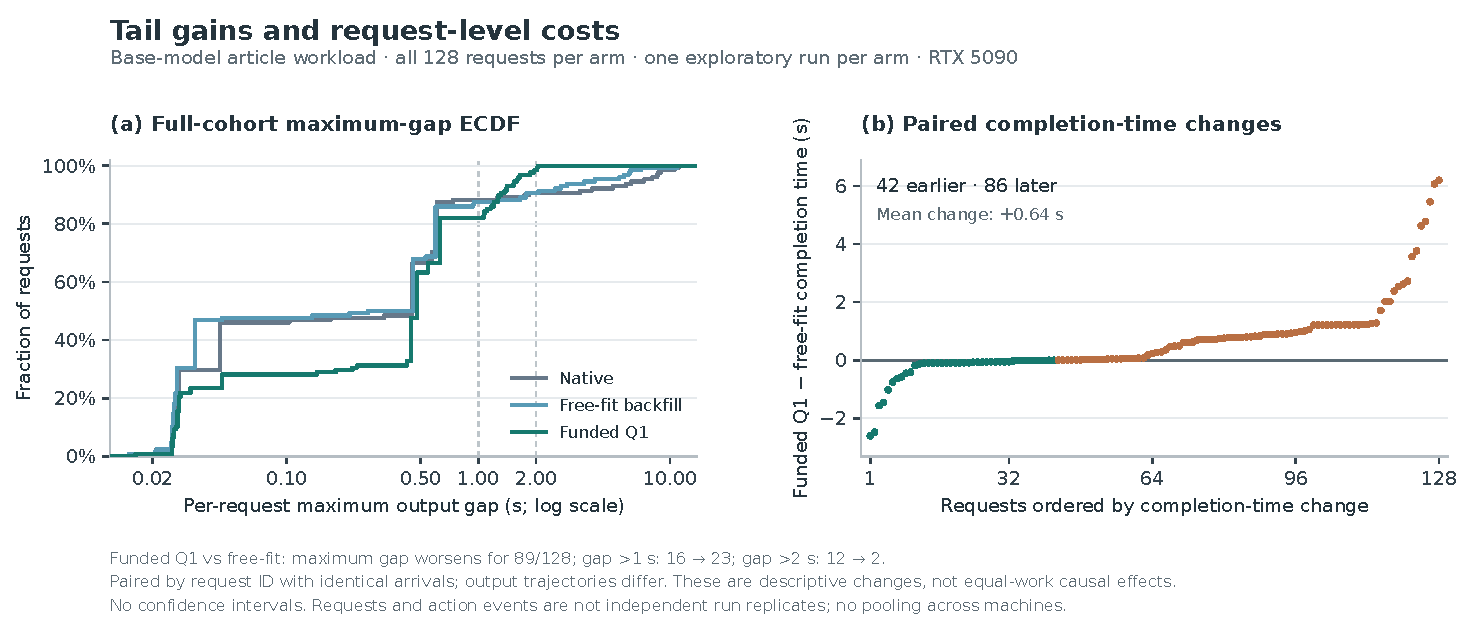
\includegraphics[width=\linewidth]{../output/strong_full_cohort_distribution.pdf}
\caption{Strong-baseline full-cohort costs. A shorter extreme pause tail coexists with worse moderate gaps and completion delays. Paired requests share inputs, not necessarily generated token sequences or scheduling histories.}
\label{fig:costs}
\end{figure}

Flow worsens for 86/128 requests versus ordinary, including five by more than four seconds. Request suffix 0049714 finishes 6.196 seconds later and its maximum gap grows from 0.027 to 1.412 seconds. Suffix 0050783 receives its first output 12.586 seconds later and finishes 4.774 seconds later, despite its subsequent maximum gap falling from 2.908 to 0.046 seconds. Both emit 1,024 tokens, but their sequences differ. These are observed harms, not causal assignments to particular recovery events.

\paragraph{Adaptive superiority does not persist across runs.}
In lease R01, executed in Q1/fixed4/adaptive order on the common path, the arms have P95 gaps 2.002/1.492/1.708 seconds, actual rates 1555.0/1553.4/1537.8 tokens/s, and mean flows 35.042/35.264/35.387 seconds. Fixed4 improves the Q1 tail at 0.10\% lower rate and 0.63\% higher mean flow. Adaptive is worse than fixed4 on P95, maximum gap, output rate and mean flow in this run.

R02 reverses serial order to adaptive/fixed4/Q1 on the same input and completes all 128 requests in every arm. In Q1/fixed4/adaptive order, P95 gaps are 1.682/1.570/1.401 seconds, actual rates 1571.2/1547.8/1559.3 tokens/s, and mean flows 34.708/35.345/35.917 seconds. The adaptive/fixed4 P95 and throughput rankings reverse; adaptive mean flow remains worse, by 0.35\% in R01 and 1.62\% in R02. Two opposite-order groups do not isolate order effects, sampling variability, or output-trajectory effects. Neither consistent failure nor stable superiority is established, and the runs are too few for a reliable uncertainty estimate.

Adaptive versus fixed4 delays completion for 56/128 requests in R01 and 91/128 in R02 (72 and 37 finish earlier); it wins/loses 9/11 and 11/9 fixed goodput points. The worst R01 flow loss, suffix 0047846, is 18.474 seconds with TTFT 16.908 seconds later, despite identical 1,024-token sequences. In R02, suffix 0052593 loses 16.760 seconds of flow and 15.435 seconds of TTFT; both outputs have 1,024 tokens but sequences differ. Even the identical-sequence case has a different scheduling history, not a shared pre-action state. These full-cohort costs motivate examining peer displacement and remaining work; event counts alone do not explain them.

\begin{figure}[t]
\centering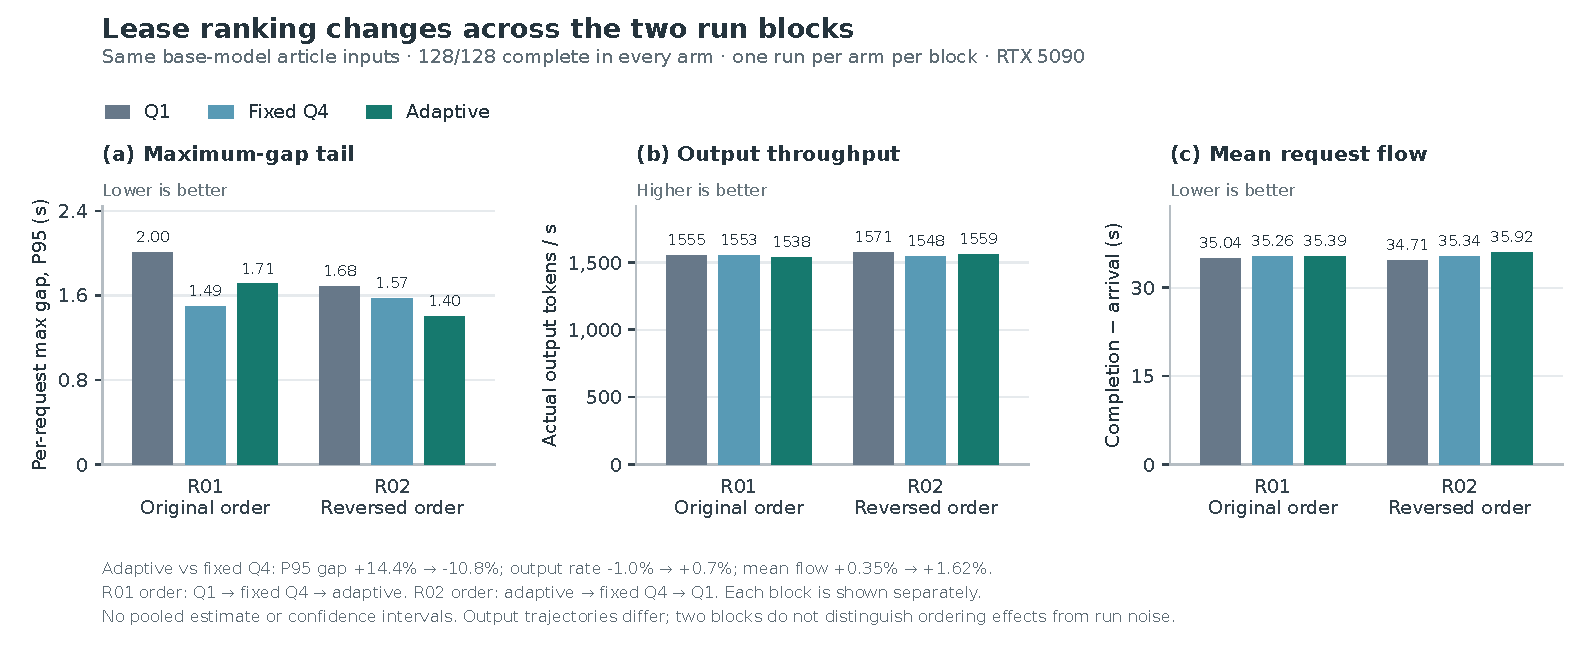
\includegraphics[width=\linewidth]{../output/lease_repeat_comparison.pdf}
\caption{Two complete lease run groups on the same article input, with reversed serial order: Q1/fixed4/adaptive in R01 and adaptive/fixed4/Q1 in R02. Adaptive versus fixed4 reverses its P95-gap and throughput rankings; mean flow is worse in both groups. Bars retain each run separately, with no pooling or confidence intervals. Two groups cannot separate run-order, trajectory and other run-level effects.}
\label{fig:repeat}
\end{figure}

The R01 action joins show real execution: Q1 has 35 one-output leases. Fixed4 has 94 leases, with 83 yielding four outputs; four leases release early at the peer-age frontier. Adaptive has 104 leases and selects $q=1,2,3$ in 14, six and 84 cases. Of its 90 multi-output choices, 89 produce multiple outputs and 88 reach the chosen quantum; the other two release after one and two outputs at the peer frontier. Desired $q$ stays at three for all 103 known-cost decisions in R01 and all 75 in R02; each run starts with one unknown-cost Q1 choice. Actual quantum variation comes from constraints, not a varying cost-derived target. Median host-overhead proxies are 32.73/32.39 ms in R01/R02 and prior decode intervals are about 15.04 ms, consistent with this constant target. The rule uses rolling medians, not each individual sample ratio; these admission/interference-inclusive proxies do not identify a causal reason for the performance ordering.

For these R01 actions, raw output/preemption joins and native plan receipts agree on release counts, endpoint growth, ownership reservations and execution. No protected target is actually preempted during its lease, and no unplanned same-call preemption appears. Q1/fixed4/adaptive have 34/94/102 forced-victim receipts and 32/72/75 actual peer-admission receipts; every such victim and admitted peer later outputs and completes. Total preemptions are 94/180/192. These receipts establish execution and recovery, not absence of peer latency harm or amortized run-level benefit. Native scheduled-token receipts are not an independent device kernel trace.

R02 action joins also pass for all three arms. Adaptive selects $q=1,2,3$ in four, five and 67 leases; 73 release at the output goal, two at the peer-age frontier and one on termination. Q1/fixed4/adaptive incur 109/171/150 actual preemptions and 35/87/75 forced rotations. Again, all forced victims and admitted peers subsequently output and complete, with no protected-target preemption. The change in event counts is descriptive and supplies no independent replication.

\section{Quality, cost, and comparison boundaries}
\paragraph{Natural endings do not imply quality equivalence.}
Three OLMoE-Instruct task domains use a 512-output cap and independent reference answers (Table~\ref{tab:quality}). Every request ends by natural EOS and none hits the cap, but holdout quality and output sequences differ across arms. All domains have zero recovery-policy actions, so none establishes the benefit or task-quality effect of a recovery quantum.

\begin{table}[t]
\centering\small
\setlength{\tabcolsep}{4pt}
\caption{Natural-ending task domains. Values are per arm: dev4096 lists Q1/fixed4/adaptive; both 512-block groups list native/ordinary/Q1/fixed4/adaptive. EOS and exact match (EM) are out of 16; token counts are actual complete outputs. No arm has a cap ending or recovery lease.}
\label{tab:quality}
\begin{tabular}{lcrrrrc}\toprule
Domain / KV blocks & Arms & EOS & EM & Output tokens & Preempts & Leases\\\midrule
Dev burst / 4096 & 3 & 16 each & 7 each & 1541 each & 0 each & 0\\
Dev burst / 512 & 5 & 16 each & 8 each & 1426 each & 1 each & 0\\
Holdout steady / 512 & 5 & 16 each & 10/8/8/9/8 & 1348/1266/1266/1265/1281 & 2/2/2/2/1 & 0\\\bottomrule
\end{tabular}
\end{table}

Development outputs are identical across arms within each block. Between the 4,096-block observer-off Q1 and 512-block observer-on Q1, 9/16 sequences change and exact match rises from 7/16 to 8/16; observer, capacity and run conditions differ, preventing a causal pressure-only comparison. The 4,096-block runs last roughly 2.14--2.18 seconds at 720.9/709.4/707.2 tokens/s. At 512 blocks, actual rates are 437.3/434.7/437.1/438.4/448.2 tokens/s, mean flows 2.567/2.583/2.564/2.559/2.495 seconds, and P95/max gaps 0.558/0.567/0.563/0.563/0.553 seconds. These short runs do not isolate installed-policy overhead. Logged development JIT warnings precede measurement, during warmup.

The independent holdout contains task IDs 48--63 arriving every 0.2 seconds. Each non-native arm preserves only 6/16 native token sequences; ordinary/Q1/fixed4/adaptive change five/five/four/five parsed answers and score one or two fewer correct answers than native. Actual rate is 391.4 tokens/s for native versus 326.1--327.4 for the other arms; mean flow is 1.334 versus 1.906--1.934 seconds. P95/max gaps stay within 0.552--0.575 seconds, below the one-second recovery trigger. We retain these observed quality and service losses. With no backfill/lease actions, different generated work and one ordered run block, they are neither evidence of quality equivalence nor a causal estimate of adaptive-quantum harm.

\paragraph{Measured transfer work in task runs.}
The dev512 arms each record 1,239,416,832 loaded bytes across 15 records and 402,653,184 stored bytes across 104 records. Native load/store copy-work sums are 0.02224--0.02279/0.00886--0.00899 seconds. Holdout load volume spans 1.313--1.416 billion bytes across 16--17 records and store volume 369.1--379.6 million bytes across 96--101 records; combined native copy-work sums are 32.01--34.60 ms. Both groups have complete observations with no missing acknowledgments or observer errors. Totals cover capture plus drain: ordinary and Q1 holdout arms each complete one 2 MiB store during drain; other holdout arms and all dev512 arms require no additional drain calls. Copy work may overlap and is not exposed request delay. Different output traces prevent interpreting lower transfer volumes as higher policy efficiency.

\paragraph{Incomplete cost and quality accounting.}
The strong article block caps 123/124/124 requests for native/ordinary/funded Q1; lease R01 caps 123/124/123 and R02 caps 123/124/124 for Q1/fixed4/adaptive. Funded versus ordinary changes 63 sequences and one output count. In the strong block, suffix 0044036 emits 173 tokens and stops under native but reaches 1,024 under ordinary and funded Q1; its longer flow is not an equal-work scheduling penalty. Article task quality is unmeasured.

Actual output rate includes the complete request-capture interval, excluding model initialization and application warmup. R01 lease chooser host elapsed times are 3.65/9.22/10.40 ms for Q1/fixed4/adaptive; these timers do not measure full scheduler/controller overhead or thread CPU time. Article performance captures lack worker transfer-byte and copy-time counters, exposed transfer delay, and live KV occupancy time series. Endpoint memory snapshots are neither traffic volume nor occupancy peaks. Host recovery intervals must not be added to overlapping transfer or execution timers. Full cost decomposition remains unavailable.

\paragraph{Prior actions and claim boundary.}
CacheOPT~\cite{cacheopt} includes urgency, memory funding, shared reservation, swap/recompute costs and predicted releases. UniBoost MemGuard~\cite{uniboost} protects service to geometric attained-decode thresholds to amortize KV movement, checking KV needs and victim swap costs. LTR~\cite{ltr} combines starvation priority with a fixed quantum counted in scheduled iterations; BidKV's pinned selector~\cite{bidkv} combines computed work, progress and accumulated preemptions, with candidates supplied by the host. Cost-aware quanta, protection and resource reservation are not individually new.

The tested distinction is an executable quantum endpoint reservation coupled to current peer constraints and compatible native admission. Fixed4 is the direct simple control; the reversal between run groups leaves stable adaptive superiority unsupported. Ordinary backfill is not a full CacheOPT/UniBoost reproduction, and no full upstream prior system is evaluated here. Any future MemGuard component comparison must preserve absolute attained-output geometric boundaries and be labeled as a component adaptation; code-version and host-loop differences prevent a full-reproduction claim.

\section{Decision and remaining evidence}
The source artifacts retain the historical residency join, frozen native packages, raw sessions, complete-cohort service reports, lease-action joins, strict task-quality evaluator and figure generators~\cite{local}. The completed native checks support the conditional resource/execution mechanism beyond CPU-only tests. They do not establish an independent adaptive contribution.

The current $h/d$ formulation is stopped as a development direction: it has not demonstrated stable superiority over fixed4, its desired quantum is constant after initialization in both runs, and completion-flow costs persist in both observed comparisons. This decision is limited to the tested cost-ratio rule and regime; it does not reject recovery leases or variable service quanta in general. The next question is what observable information about victim/peer displacement and remaining work is needed to explain or improve complete-cohort outcomes. No replacement controller is implemented or claimed here.

The completed independent holdout adds natural-ending and transfer evidence and exposes quality variability; it does not activate the recovery mechanism. Recovery-active natural task cohorts, other input domains, component ablations, and enough run-level repeats to quantify uncertainty remain missing evidence. No further experiment is running at this checkpoint. The demonstrated artifact is a native resource/execution mechanism with an explicit local progress condition and measured service tradeoffs, not a completed method paper.

\begin{thebibliography}{9}
\small
\setlength{\itemsep}{2pt}
\setlength{\parskip}{0pt}
\bibitem{cacheopt} CacheOPT, version 2. \url{https://arxiv.org/abs/2503.13773}.
\bibitem{uniboost} UniBoost. \url{https://yl3469.github.io/uniboost-icml26/}; paper version 1, \url{https://arxiv.org/abs/2606.18431}.
\bibitem{ltr} LTR, version 1, Algorithm 1. \url{https://arxiv.org/abs/2408.15792}.
\bibitem{bidkv} BidKV selector, pinned commit \texttt{5ee8025}. \url{https://github.com/vLLM-HUST/vllm-ascend-hust-bidkv/blob/5ee80256d263d58b1e512d9d436d47e9bac564ba/vllm_ascend_bidkv/selector.py}.
\bibitem{local} A-line evidence and reproduction index, 2 October 2026. \path{recovery_quantum_20261002/README.md}. Frozen sources, raw sessions, analyses, costs, plots and the decision record.
\end{thebibliography}
\end{document}
